% This is part of Un soupçon de mathématique sans être agressif pour autant
% Copyright (c) 2015
%   Laurent Claessens
% See the file fdl-1.3.txt for copying conditions.

%--------------------------------------------------------------------------------------------------------------------------- 
\subsection*{Activité : étiquette d'une boîte de conserve}
%---------------------------------------------------------------------------------------------------------------------------

\begin{wrapfigure}[3]{r}{6.0cm}
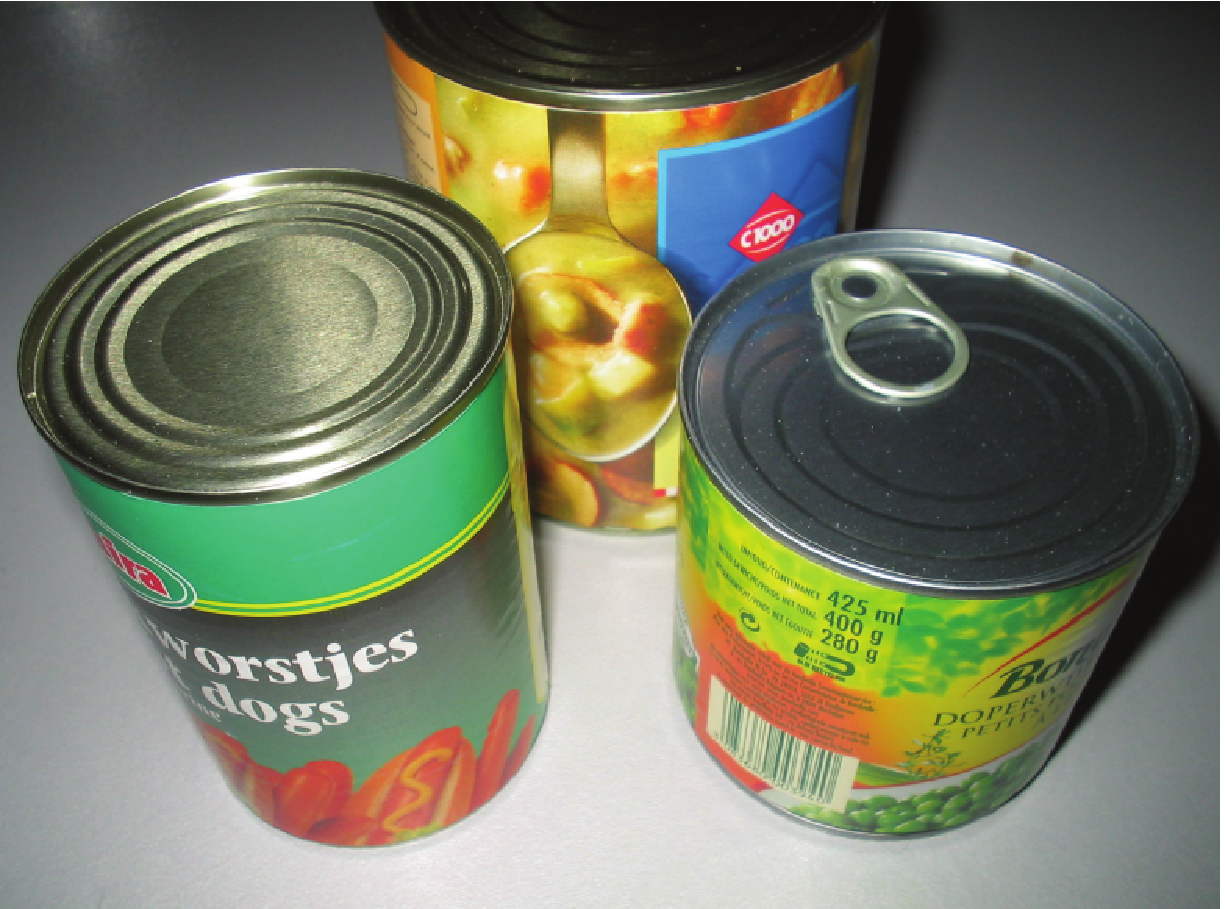
\includegraphics[width=6cm]{conserve.pdf} 
\end{wrapfigure}


Une boîte de conserve a souvent une forme de cylindre. Combien de face est-ce qu'une telle boîte possède ?

\begin{enumerate}
    \item
        Si on décolle l'étiquette, quelle forme a-t-elle ?
    \item

 Si on ouvre une boîte de conserve des deux côtés et qu'on la déplie, on obtient le patron d'un cylindre de révolution. À main levée, tracer un tel patron.
 \item
    Déterminer le périmètre de la base en fonction du rayon de cette base. En déduire la longueur de la face latérale. 
\item

    Réaliser le patron d'un cylindre de révolution de hauteur \SI{5}{\centi\meter} ayant pour base un disque de rayon \SI{3}{\centi\meter}. 

\end{enumerate}
